\chapter{结合图路径和局部邻域的Transformer模型}

% 本章主要对结合图路径和局部邻域的Transformer模型TKGE-PN的总体设计和模块的具体实现进行了介绍。主要包括对基于图神经网络的方法以及NATLP模型存在问题的分析、模型的总体框架设计、基于有偏随机游走的图路径采样算法的设计、Path-Transformer路径编码模块以及Neighbor-Transformer局部邻域编码模块的具体设计。

本文先前提出的NATLP模型将Transformer模型应用于知识图谱补全任务,通过关系特定的邻居实体信息构造和邻域感知Transformer模块解决了关系建模以及图结构学习的问题,提高了模型的表达能力,获得了优异的知识图谱补全性能,但是由于主要利用局部邻域信息进行预测,和基于图神经网络的方法类似,依然存在对图谱中长距离依赖学习不足的问题。针对以上问题,本文基于前文提出的NATLP模型,尝试利用知识图谱的图路径结构来学习图谱中的长距离依赖,进一步提出了提出了一种基于Transformer的结合图路径和局部邻域的知识图谱嵌入方法(A Transformer-based Knowledge Graph Embedding Model Combining Graph Paths and Local Neighborhood,TKGE-PN)。此外,为了验证本文提出的TKGE-PN算法能够通过结合图路径和局部邻域信息实现对知识图谱中的长短距离依赖的综合学习,提高链路预测任务的性能表现,本文在两个基准数据集上对TKGE-PN进行了实验验证。首先说明了用来对比的基线算法以及模型在两个数据集上的超参数设置,随后介绍了模型的整体实验结果并进行了深入的探究,最后通过消融实验对模型的关键设计进行了分析和讨论。

\section{现有问题分析}
NATLP模型将Transformer模型应用到了知识图谱补全任务中,对传统的Transformer模型的自注意力机制的计算方式进行改进,捕获了中心实体局部邻域内的结构信息,学习到了邻居实体之间的相互依赖,解决了先前基于图神经网络的方法模型表达能力差、对邻居实体之间相互依赖学习不足的问题,获得了很大的性能提升。

但是,NATLP模型依然存在缺陷。和图神经网络类似的是,NALTP同样基于中心实体的局部邻域进行知识图谱补全,想要学习多跳之外的邻居信息就需要进行多层网络的堆叠,这会导致模型遭遇过度平滑问题,因此模型并没有解决基于图神经网络的知识图谱嵌入方法对于长距离依赖学习不足的缺点。在知识图谱中,长距离的含义是实体间通过边连接需要经过多个中间节点。长距离依赖反映的是实体之间较为间接的联系,这种联系在理解实体间复杂关系的层面上是非常重要的。例如,某一个历史人物与某一个现代组织之间可能存在某种长距离的关联,尽管他们之间直接的联系很少,但通过一系列历史事件和影响,可以构建出两者之间的联系,因此捕捉长距离依赖有益于推理和查询知识图谱的高阶模式。

基于图神经网络的方法主要是通过利用中心实体的局部邻域中蕴含的信息来完成知识图谱的补全。每层图神经网络只能学习到中心实体的一跳邻居的信息,这导致模型能够很好的捕捉知识图谱中的短距离依赖,而对于实体和实体之间的长距离依赖的学习不够充分。虽然其可以通过堆叠多层图神经网络让中心实体感知到距离更远的其他实体,但这样的方式只在层数较低(例如一到两层)时有效,之后随着网络层数的进一步增加,模型的性能反而会出现快速下降的情况,这主要是由于过度平滑问题(over-smoothing)所导致的,即因为模型感受野的重叠而导致不同节点的表示过于相似无法进行区分。文献\cite{over-smoothing}对这种现象进行了系统和定量的研究,通过引入定量指标,发现导致过度平滑的关键因素是中心节点接收到的有效信息与噪声比例过低,结果如图\ref{information-noise}所示,该图来自于文献\cite{over-smoothing}原文。在每层图神经网络中,节点都会聚合其所有邻居节点的信息并传递给下一层,这导致最后一层图神经网络引入了大量的噪声信息。因此基于图神经网络的方法一般只能捕捉单个实体附近1-2跳内的局部邻域信息,而缺乏利用长距离乃至全局信息的能力。
\begin{figure}[htb]
  \centerline{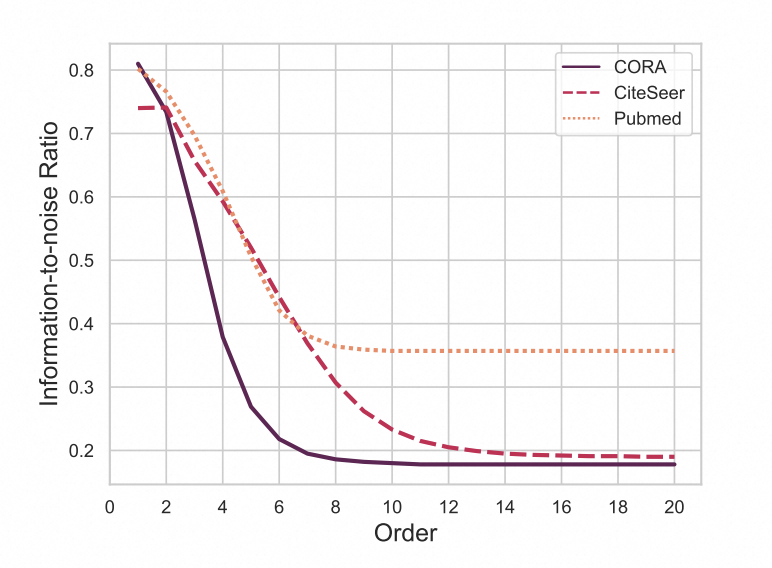
\includegraphics[width=0.5\textwidth]{pic/information-noise.png}}
  \caption{网络层数对信噪比的影响}
  \label{information-noise}
\end{figure}

为了解决以上问题,本文尝试引入知识图谱图路径信息学习知识图谱中的长距离依赖,在NATLP模型的基础上,进一步提出了一种基于Transformer的结合图路径和局部邻域的知识图谱嵌入方法(A Transformer-based Knowledge Graph Embedding Model Combining Graph Paths and Local Neighborhood,TKGE-PN)。基于图神经网络的方法的成功证明了实体的局部邻域蕴含了丰富的信息,但知识图谱的结构信息除了图神经网络使用的局部邻域之外还有多种其他的表达形式,例如图路径以及子图。在知识图谱中,图路径被定义为图谱中的实体-关系链,由不同的三元组首尾相连所组成,例如(Yao Ming, Born In, Shanghai, City Of, China)。相比于局部邻域,图路径的形势天然适合学习远距离的关系,能够帮助模型更好地捕获实体和实体之间长距离的依赖,如图\ref{long-term-dependency}所示。在现有的知识图谱嵌入方法中,便有不少研究尝试通过图路径信息来学习图谱中的长距离依赖,例如RSN\cite{RSN}和Interstellar\cite{Interstellar},但这些方法却忽略了中心实体丰富的局部邻域,在近距离依赖的学习上有着很大的不足。因此,本文尝试结合图路径和局部邻域两类图结构信息,使得模型能够在更好地学习长短距离依赖的同时避免过度平滑问题的出现。同样的,和NATLP模型类似的是,和图神经网络浅层的网络结构以及简单的信息聚合方式相比,Transformer的自注意力机制能够给模型带来更强大的表达能力。本文提出的TKGE-PN模型以中心实体作为起点,首先采用有偏随机游走算法对图路径进行采样,并通过基于Transformer的图路径编码模块Path-Transformer学习图路径中的语义信息并转化为向量表示,最后通过Neighbor-Transformer局部邻域编码模块将图谱中的长距离和短距离依赖进行结合。此外由于相比于近距离的信息,长距离信息反映的是实体之间间接的联系,学习更为困难,因此针对这个问题,本文在Path-Transformer图路径编码模块中设计了一个掩蔽实体关系预测任务,以确保模型能够充分学习图路径之间的长距离依赖。

\begin{figure}[htb]
    \centerline{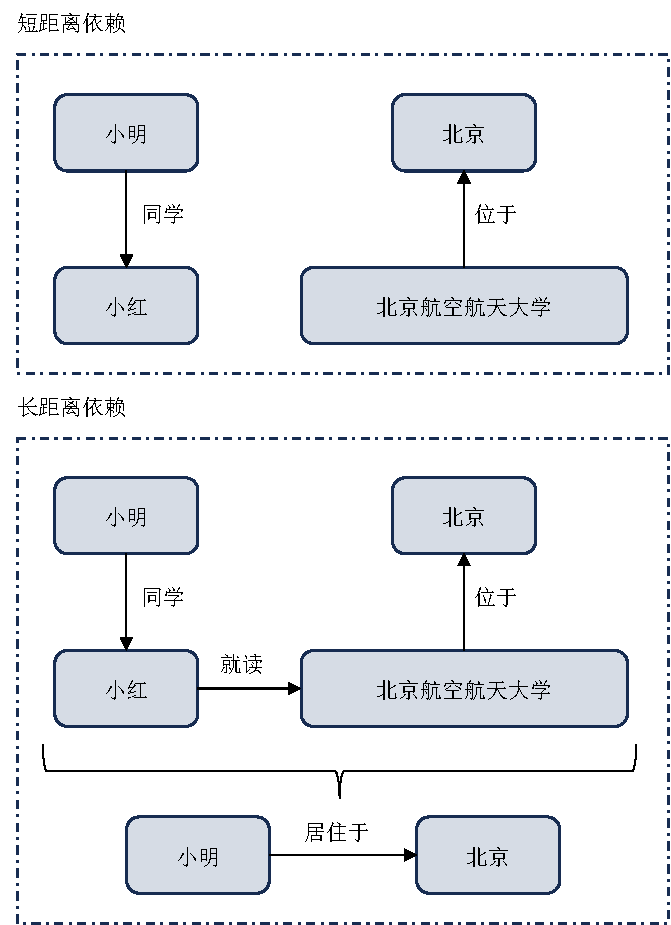
\includegraphics[width=0.5\textwidth]{pic/long-term-dependency.pdf}}
    \caption{知识图谱中的短距离信息和长距离信息}
    \label{long-term-dependency}
  \end{figure}

\section{TKGE-PN模型设计}

\subsection{符号定义}
为了方便说明论文提出的TKGE-PN模型的实现细节,本节对TKGE-PN模型中的关键概念和相关的数学符号进行了定义,具体内容参见表\ref{definition_TKGE-PN}。

\setlength{\tabcolsep}{20pt}

\renewcommand\arraystretch{1.2}
\begin{longtable}[htbp]{cc}
  % 首页表头
  \caption{TKGE-PN模型中的符号定义}
  \label{definition_TKGE-PN}\\
  \toprule
  符号  & 说明\\
  \midrule
  \endfirsthead
  % 续页表头
  \caption{TKGE-PN模型中的符号定义}\\
  \toprule
  符号  & 说明 \\
  \midrule
  \endhead
  % 首页表尾
  \hline
  % \multicolumn{2}{r}{\small 续下页}
  \endfoot
  % 续页表尾
  \bottomrule
  \endlastfoot
  
  $\mathcal{G}$   &   知识图谱      \\
  $\mathcal{E}, \mathcal{R}, \mathcal{T}$   &   实体集合、关系集合、边集合      \\
  $\mathcal{G}^\prime$  &  拓展后的知识图谱      \\
  $\mathcal{R}^{\prime}$   &   拓展后的关系集合      \\
  $\mathcal{T}^{-1}$   &   逆关系边集合      \\
  $\mathcal{T}^{\prime}$   &   拓展后的边集合      \\
  $(s,r,?)$  &   待遇测的三元组      \\
  $s$   &   头实体即中心实体      \\
  $o$   &   尾实体即目标实体      \\
  $e$   &   实体      \\
  $r$   &   关系      \\
  $r^{-1}$   &   关系$r$的逆关系      \\
  $\boldsymbol{s},\boldsymbol{o}$ & 头实体嵌入和尾实体嵌入\\
  $\boldsymbol{e},\boldsymbol{r}$ & 实体嵌入和关系嵌入\\
  $T$ & 图路径的长度\\
  $P$ & 知识图谱中的图路径\\
  $\mathcal{N}_s$ & 实体 $s$的一阶邻居节点集合\\
  $\mu_{depth}(e_{i+1})$ & 候选实体$e_{i+1}$的深度偏差\\
  $\mu_{degree}(e_{i+1})$ & 候选实体$e_{i+1}$的度数偏差\\
  $\alpha$ & 控制深度偏差的权重\\
  $\beta$ & 控制度数偏差的权重\\
  $p_{sample}$ & 采样过程中实体被选中的概率\\
  $e_m,r_m$ & 掩蔽实体关系预测任务中被掩蔽的实体或关系\\
  $\mathbf{M}_{input}^{P},\mathbf{M}_{output}^{P}$ & Path-Transformer模块的输入和输出\\
  $\boldsymbol{e}_{mask}$ & 掩蔽占位嵌入\\
  $\boldsymbol{e}_{query}$ & 查询向量\\
  $d$ & 嵌入维度\\
  $\phi_{chk}$ & 棋盘式特征重组\\
  $\circledast$ & 循环卷积操作\\
  $f(\cdot )$ & ReLU激活函数\\
  $vec(\cdot)$ & 二维张量转化为一维向量\\
  $\omega_r$ & 特定于关系$r$的卷积层参数\\
  $\mathbf{W}_r$ &特定于关系$r$的全连接层参数\\
  $\boldsymbol{e}_{cls}$ & Path-Transformer特殊嵌入Class Token\\
  $\boldsymbol{e}_{gcls}$ & Neighbor-Transformer特殊嵌入Global Class Token\\
  $\mathbf{TE}$ & 类型嵌入\\
  $\mathbf{PE}$ & 位置嵌入\\
  $a_{ij}$ & 第i个输入和第j个输入之间的注意力得分\\
  $dis(e_i,e_j)$ & 实体$e_i$与实体$e_j$之间最短路径的距离\\
  $deg(e)$ & 实体$e$的节点度数\\
  $\boldsymbol{o}_t$ & 模型预测的候选实体的嵌入\\
  $\sigma $ & sigmoid激活函数\\
  $p$ & 三元组正确概率\\
  $L_{MERP}$ & 掩蔽实体关系预测任务的损失\\
  $L_{LP}$ & 链路预测任务损失\\
  $L$ & 模型损失\\
  $t_i$ & 第i个三元组的标签\\

\end{longtable}

和NATLP中的处理方式类似的是,为了确保不同实体之间信息的双向流动,TKGE-PN会对原始的知识图谱进行拓展,为知识图谱中的每个事实三元组$(s,r,o)$添加对应的逆关系$r^{-1}$和逆三元组$(o,r^{-1},s)$:
% \begin{equation}
%   \mathcal{R}^{\prime}=\mathcal{R}\cup\{ r^{-1} | r\in \mathcal{R}\}
% \end{equation}
% \begin{equation}
%   \mathcal{T}^{-1}= \{ (o,r^{-1},s)| (s,r,o)\in \mathcal{T}\}
% \end{equation}
% \begin{equation}
%   \mathcal{T}^{\prime} = \mathcal{T}\cup\mathcal{T}^{-1}
% \end{equation}
% \begin{equation}
%   \mathcal{G}^\prime = (\mathcal{E}, \mathcal{R}^\prime, \mathcal{T}^\prime)
% \end{equation}
\begin{gather}
    \mathcal{R}^{\prime}=\mathcal{R}\cup\{ r^{-1} | r\in \mathcal{R}\}\\
    \mathcal{T}^{-1}= \{ (o,r^{-1},s)| (s,r,o)\in \mathcal{T}\}\\
    \mathcal{T}^{\prime} = \mathcal{T}\cup\mathcal{T}^{-1}\\
    \mathcal{G}^\prime = (\mathcal{E}, \mathcal{R}^\prime, \mathcal{T}^\prime)
\end{gather}

\subsection{模型总体结构}

本节主要对提出的基于Transformer的结合图路径和局部邻域的知识图谱嵌入方法TKGE-PN的总体结构进行介绍。模型整体架构如图\ref{TKGE-PN_architecture}所示。

和NATLP不同的是,TKGE-PN模型并没有采用传统的编码器-解码器架构,而是利用Transformer自身的强大表达能力直接对目标实体的嵌入进行预测。相比于原先的方法,这样的架构最大的优点是模型可以充分发挥Transformer自注意力机制的强大表达能力,其性能不会被用作解码器的基于卷积神经网络的知识图谱嵌入方法所限制。

TKGE-PN模型主要由三个核心部分组成。首先第一部分是基于有偏随机游走的图路径采样算法,主要职责是以中心实体为起点在图谱中采样多条图路径;随后第二部分Path-Transformer路径编码模块负责学习采样到的图路径中蕴含的长距离的语义信息并将其转换为向量表示;最后Neighbor-Transformer局部邻域编码模块接收来自Path-Transformer的输入,整合待预测事实三元组中的信息以及多条图路径所构成上下文邻域信息,实现图路径以及局部邻域结构信息的结合,并以此预测事实三元组的得分。

\begin{figure}[htbp]
  \centerline{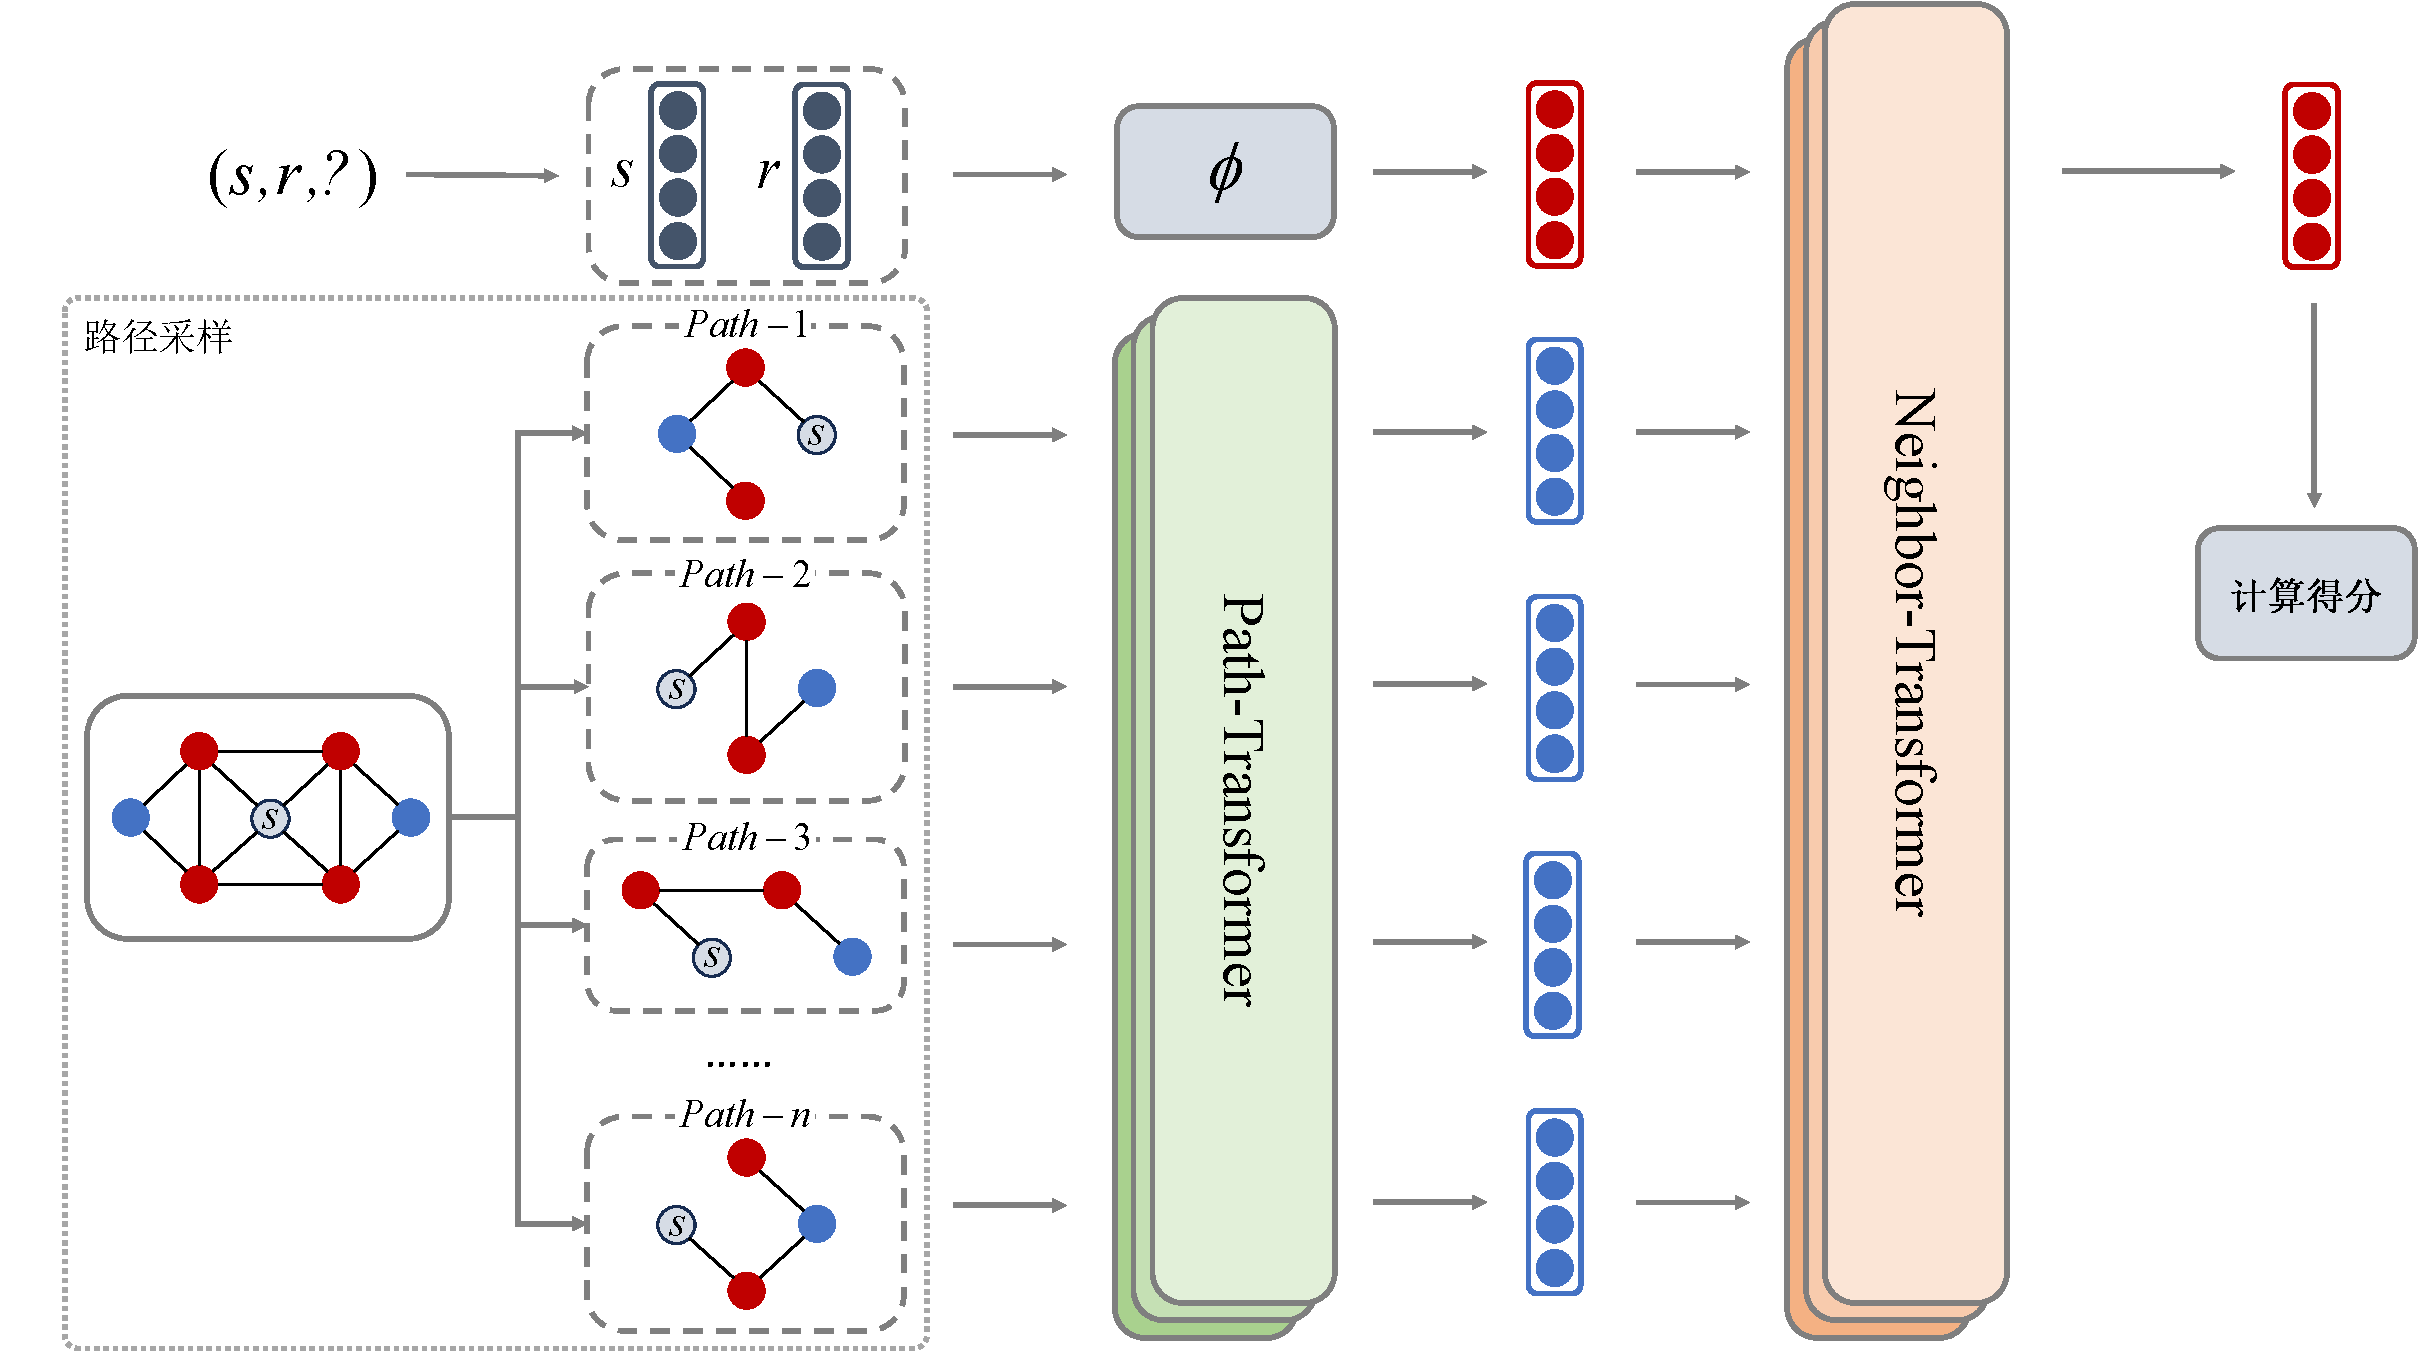
\includegraphics[width=0.9\textwidth]{pic/TKGE-PN.pdf}}
  \caption{TKGE-PN模型整体架构}
  \label{TKGE-PN_architecture}
\end{figure}

\subsection{基于有偏随机游走的图路径采样算法}

为了通过图路径来学习实体之间的长距离依赖,TKGE-PN模型的第一个任务是获得知识图谱中的图路径信息。由于知识图谱的规模往往十分庞大,因此遍历图谱中所有可能的图路径组合是一件不可能的工作。因此模型需要对图路径进行有选择的采样。为了让模型能够充分利用图路径信息,提高链路预测的准确性,如何采样到高质量的知识图谱图路径是TKGE-PN首先需要解决的问题。

给定一个待预测的三元组$(s,r,?)$,图路径采样模块的主要任务是获得一条或者若干条以头实体$s$为起点的图路径用于链路预测任务。在TKGE-PN模型中,知识图谱中的图路径被定义为图谱中的实体-关系链,在链中实体和关系交替出现,链的第一个元素和最后一个元素必须为实体,例如(Yao Ming, Born In, Shanghai, City Of, China)。在图谱中,以节点$s$为起点,长度为$T$的图路径$P$表示为以下形式:

\begin{equation}
  \begin{aligned}
     &P=<s,r_1,e_1,r_2,e_2,...,r_T,e_T>, \\
     &{\forall}i \in (0,T),e_i\in\mathcal{E},r_i\in\mathcal{R}^{\prime},(e_i,r_{i+1},e_{i+1})\in\mathcal{T}^{\prime}
  \end{aligned}
\end{equation}

以往的基于图路径的知识图谱嵌入方法在给事实三元组打分时对于单个样本所采样的图路径数量往往只有1-2条,例如RSN\upcite{RSN}和Interstellar\upcite{Interstellar}。这些方法采样到的图路径数量相比于知识图谱中可能的图路径数量是十分有限的,因此模型从这些图路径中学习得到的信息往往是片面的,很难全面地挖掘到中心实体对其他实体的长距离依赖,特别是当中心实体的节点度数比较高时,这样的问题会更加严重。此外,并不是所有的图路径都对高质量的知识图谱嵌入有意义,部分低质量的图路径信息中的实体和关系组合可能缺乏明确的含义,会引入额外的噪声,反而降低模型的性能。为了解决以上提到的这些问题,本文提出了一种基于有偏随机游走的图路径采样算法。

首先,为了解决图路径采样数量不足导致模型学习到的信息不够全面的问题,对于一个待预测的三元组$(s,r,?)$,TKGE-PN的图路径采样模块不再采样固定数量的图路径,而是选择将图路径采样数量设置为头实体$s$的节点度数的值。这样做的基本思路是,一般来说,实体的节点度数越高,以实体作为起点可能采样到的图路径就越多,该实体和其他实体之间可能存在的长距离的依赖就越丰富,因此需要采样更多的图路径;而当节点度数较小时,中心实体可能存在的长距离依赖相对较少,采样一到两条图路径就能够实现充分的学习。因此随实体节点度数动态变化的图路径采样条数有利于更加全面、高效的捕捉图谱中的长距离依赖信息。

此外,为了避免随机采样的图路径之间出现路径重复而导致信息冗余的情况,对于同一个头实体节点$s$,TKGE-PN的采样算法会确保采样到的不同图路径中的前三个元素组成的事实三元组唯一,即对于不同图路径$P_i=<s,r_1^{i},e_1^{i},...,r_T^{i},e_T^{i}>$和$P_j=<s,r_1^{j},e_1^{j},...,r_T^{j},e_T^{j}>$,有$(s, r_1, e_1)\neq(s, r_2, e_2)$,其中$e_1^{i},e_1^{j}\in \mathcal{N}_s$,$\mathcal{N}_s$为实体 $s$的一阶邻居节点组成的集合。通过这样的采样方式。模型不仅保证了采样到的图路径之间有足够的区分度,还让采样到的路径覆盖了中心实体的一阶邻域。基于所有这些采样到的图路径,模型就能学习到中心实体的局部邻域信息,实现长短距离依赖的同时学习。

为了确保采样到的图路径能够帮助模型进行知识图谱补全,TKGE-PN的图路径采样模块采用有偏随机游走算法来决定图路径中每一跳选中的实体和关系,实现高质量的图路径采样。为了能够更好的捕获长距离的依赖,TKGE-PN希望采样到的路径能够尽可能地远离起始的头实体,即采样深度更大一些。为了实现这一点,在进行路径采样的过程中,模型提出了一个深度偏差项来控制路径采样的过程。具体来说,假设在图路径采样的过程中,起始节点为$s$,当前选中的实体为$e_i$,上一跳实体为$e_{i-1}$,下一跳的候选实体$e_{i+1}$为$e_i$的一阶邻居,则深度偏差$\mu_{depth}(e_{i+1})$的计算方式为:
\begin{equation}
  \mu_{depth}(e_{i+1})=1-\alpha\cdot\frac{1}{dis(s,e_{i+1})}
\end{equation}
其中$dis(s,e_{i+1})$为实体$s$与实体$e_{i+1}$之间最短路径的距离,$\alpha$为控制采样过程中路径深度的超参数,为了获得深度更大的路径,一般设置为$\alpha>0$,这样候选实体距离起始实体的最短距离越大,则在计算采样概率时的深度偏差越大。图\ref{depth_bias}说明了一个具体的实例。

\begin{figure}[htbp]
  \centerline{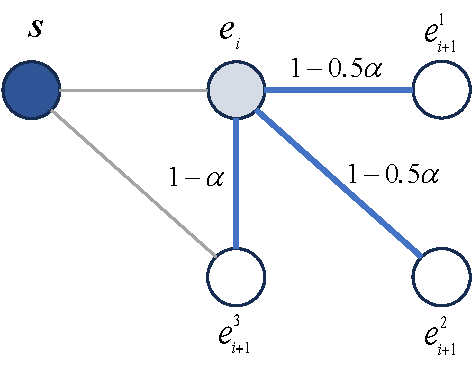
\includegraphics[width=0.4\textwidth]{pic/depth_bias.pdf}}
  \caption{图路径采样过程中的深度偏差}
  \label{depth_bias}
\end{figure}

除了路径深度之外,在图路径采样的过程中,TKGE-PN还将实体的节点度数纳入了考虑。作为知识图谱中一种重要的结构信息,实体的节点度数反映了实体在整个知识图谱中的全局重要性,实体的节点度数越高,说明该实体连接的其他实体和关系越多,蕴含的信息越丰富,应该越重要,为了提高知识图谱补全的准确性,在采样的过程中,节点度数较高的实体被采样到的概率应该越大,对应的权重应该更高。为了实现这一点,模型在路径采样过程中引入了度数偏差来进行控制。对于候选实体$e_{i+1}$,度数偏差$\mu_{degree}(e_{i+1})$的计算方式如下:
\begin{gather}
  \mu_{degree}(e_{i+1})=\lg(deg_{(e_{i+1})})
\end{gather}
其中$deg_{(e_{i+1})}$为候选实体$e_{i+1}$的度数。此外,本文认为,如果一个实体相邻的实体的节点度数很高,那么该实体的重要性应该也会受到邻居实体的影响随之增加,因为经过该节点可以获取到重要性较高的其他实体节点的信息,因此在计算度数偏差时TKGE-PN将相邻实体的节点度数也纳入了考虑,有:
\begin{gather}
  \mu_{degree}(e_{i+1})=\frac{1}{2}\lg(deg_{e_{i+1}})+\frac{1}{2\|\mathcal{N}_{e_{i+1}}\|}\sum_{e_k\in\mathcal{N}_{e_{i+1}}}\lg(deg_{e_k})
\end{gather}

最终,模型可以得到在图路径采样的过程中,下一跳候选实体$e_{i+1}$被选中的未正则化的概率,具体计算公式为:
\begin{equation}
  \mu_i = \mu_{depth}(e_{i+1})+\beta\cdot\mu_{degree}(e_{i+1})
\end{equation}
\begin{equation}
  p_{sample}(e_{i+1})=\left\{
      \begin{aligned}
          &\mu_i &&\quad (e_i,r_i,e_{i+1})\in \mathcal{T}^{\prime} \\
          &0 &&\quad otherwise
      \end{aligned}
  \right.
\end{equation}
% \begin{gather}
%   \mu_i = \mu_{depth}(e_{i+1})+\beta\cdot\mu_{degree}(e_{i+1})\\
%   p_{sample}(e_{i+1})=\left\{
%       \begin{aligned}
%           &\mu_i &&\quad (e_i,r_i,e_{i+1})\in \mathcal{T}^{\prime} \\
%           &0 &&\quad otherwise
%       \end{aligned}
%   \right.
% \end{gather}
其中$\beta$为控制采样过程中度数偏差的权重。

\subsection{Path-Transformer路径编码模块}

通过基于有偏随机游走的采样算法,TKGE-PN模型获得了若干条图路径用于链路预测任务。但是这些采样到的图路径无法直接使用,还需要Path-Transformer路径编码模块学习其中蕴含的语义信息并转换为对应的向量表示。和处理局部邻域结构不一样的是,图路径天然具有序列数据的形式,而Transformer被认为是建模序列数据的最强大的神经网络,因此原始的Transformer网络就能够很好的挖掘路径中实体与实体、实体与关系之间的长短距离依赖,而无需对网络结构进行额外的改造。

给定一条长度为$T$的图路径$P=<s,r_1,e_1,...,r_T,e_T>$,Path-Transformer路径编码模块的输入主要由以下几个部分组成:图路径嵌入表示$\mathbf{M}_{path} $,以及一个可学习的特殊嵌入Class Token的向量表示$\mathbf{e}_{cls}$用于获取所有输入的统计特性,因此路径编码模块的输入表示为:
\begin{gather}
  \mathbf{M}_{path} = [\boldsymbol{e}_s,\boldsymbol{r}_1,\boldsymbol{e}_1,...,\boldsymbol{r}_T,\boldsymbol{e}_T]\\
  \mathbf{M}_{path}^{\prime} = [\boldsymbol{e}_{cls},\mathbf{M}_{path}]
\end{gather}
其中$\boldsymbol{e}_{cls}\in\mathbb{R}^d$,$\mathbf{M}_{path} \in \mathbb{R}^{(2T+1)\times d}$。$\mathbf{M}_{path}$由图路径中包含的所有的实体及关系对应的嵌入构成,$\boldsymbol{e},\boldsymbol{r} \in \mathbb{R}^d$ 代表分别代表实体和关系嵌入,$d$则为嵌入向量维度的大小。同样的,和NATLP类似,Path-Transformer采用类型嵌入来帮助模型区分实体嵌入,关系嵌入以及特殊嵌入向量$\boldsymbol{e}_{cls}$。此外,由于图路径是序列数据,Path-Transformer采用可学习的位置嵌入来识别图路径中实体和关系之间的顺序关系,因此Path-Transformer的最终输入表示为:
\begin{equation}
  \mathbf{M}_{input}^{P} = \mathbf{M}_{path}^{\prime}+\mathbf{TE} + \mathbf{PE}
\end{equation}
其中$\mathbf{TE}$ 为类型嵌入,$\mathbf{PE}$为位置嵌入。

在完成输入构造后,Path-Transformer会利用自注意力机制学习图路径中的语义信息。设Path-Transformer模块最后一层的输出为$\mathbf{M}_{output}^{P}\in\mathbb{R}^{(2T+1)\times d}$,TKGE-PN取输出中特殊嵌入向量$\boldsymbol{e}_{cls}$对应位置的嵌入$\boldsymbol{e}_{path}\in\mathbb{R}^d$作为当前图路径的向量表示。

Path-Transformer路径编码模块尝试从知识图谱图路径中挖掘长距离的依赖用于链路预测任务,但是相比于近距离的局部邻域,图路径中蕴含的长距离依赖反映的是实体之间间接的联系,容易在学习的过程中丢失,模型学习起来是更加困难的。针对这样的挑战,受到BERT\upcite{BERT}中掩蔽语言建模(Masked Language Model,MLM)预训练任务的启发,TKGE-PN提出了掩蔽实体关系预测(Masked Entity and Relation Prediction,MERP)任务,以加强Path-Transformer从图路径上下文中挖掘信息的能力。

具体来说,对于输入的每一条图路径$P$,模型将会随机选择遮掩或者替换掉某个关系或者实体进行预测任务。以实体为例,在掩蔽替换阶段,被选中的实体$e_m$ 将会以一定概率被替换成特殊的掩蔽占位嵌入$e_{mask}$、其他的随机实体或者维持不变,模型使用超参数来调节以上三种情况的概率。而在预测阶段,模型取Path-Transformer输出嵌入矩阵$\mathbf{M}_{output}^{P}$中被选中的实体对应的嵌入$\boldsymbol{e}_{m}^\prime$来尝试辨认出被遮掩的正确实体$e_m$。具体来说,对于一个候选的实体$e_t$,模型将$\boldsymbol{e}_{m}^\prime$通过一个双层全连接层并计算$\boldsymbol{e}_{m}^\prime$与$\boldsymbol{e}_{t}$之间的余弦相似度来获得候选实体$e_t$的正确概率$p_m$:
\begin{equation}
  p_m(e_t)=\sigma((f(\boldsymbol{e}_m^\prime\mathbf{W}^{\prime})\mathbf{W}^{\prime\prime})\boldsymbol{e}_t)
\end{equation}
其中$f (\cdot)$和$\sigma(\cdot)$分别代表ReLU和sigmoid激活函数,$\mathbf{W}^{\prime}$和$\mathbf{W}^{\prime\prime}$分别为两个全连接层的参数。当被选中的元素为关系时,处理方法类似。最后TKGE-PN通过交叉熵损失函数,计算得到掩蔽实体关系预测任务的分类损失为:
\begin{equation}
  L_{P} = -\frac{1}{N}\sum\limits_{i}t_m^ilog(p_m^i)+(1-t_m^i)log(1-p_m^i)
\end{equation}
其中$t_m^i$为MERP任务中的分类标签,$p_m^i$为对应候选实体的正确概率。

掩蔽实体关系预测任务加强了Path-Transformer挖掘图路径中语义信息的能力。在原本的训练过程中,由于近距离的依赖学习难度较低,模型可能会倾向于挖掘近距离的实体中蕴含的信息,而忽略了远距离的部分。而通过随机地对图路径中的元素进行掩蔽,模型无法再单纯地依赖某个特定的图路径元素;通过对掩蔽的元素进行预测,模型也确保了信息不会丢失。基于掩蔽实体关系预测任务,模型实现了对图路径中长短距离依赖信息的平衡。

\subsection{Neighbor-Transformer局部邻域编码模块}

给定一个待预测的三元组$(s,r,?)$,通过基于有偏随机游走的图路径采样算法,模型已经获得了以头实体$s$为起点的多条图路径,数量等于头实体$s$的节点度数。通过对采样的规则进行限制,这些图路径覆盖了头实体$s$的一阶局部邻域。因此,Neighbor-Transformer局部邻域编码模块通过基于Path-Transformer学习到的所有的图路径表示,便能够同时结合知识图谱的局部邻域结构信息和图路径结构信息,在避免过平滑问题的同时实现对于长短距离依赖的同时学习,提高知识图谱补全任务的性能。

Neighbor-Transformer局部邻域编码模块的输入主要包含以下几个部分:图路径嵌入矩阵$\mathbf{M}_{paths}$,查询嵌入$\boldsymbol{e}_{query}$以及一个可学习的特殊嵌入$\boldsymbol{e}_{gcls}$。$\mathbf{M}_{paths}\in\mathbb{R}^{N_p\times d}$由所有采样到的以头实体$s$为起点的图路径的嵌入表示组成,其中$N_p$为采样到的图路径的数量,有:
\begin{equation}
  \mathbf{M}_{paths}=\left[ \boldsymbol{e}_{P_1},\boldsymbol{e}_{P_2},...,\boldsymbol{e}_{P_{N_p}}\right]
\end{equation}
其中$\boldsymbol{e}_{P_i} \in \mathbb{R}^d$为第$i$条图路径的向量表示。为了能够发挥Transformer模型的表达能力,避免模型的性能被基于卷积神经网络的解码器限制,TKGE-PN抛弃了NALTP中采用的编码器-解码器架构,而是利用Transformer网络尝试直接拟合待预测尾实体$o$的嵌入。查询向量$\boldsymbol{e}_{query}$的主要作用是向Transformer传递待预测三元组的信息,让模型能够基于当前输入调整注意力分数的计算,提高模型链路预测的性能。$\boldsymbol{e}_{query}$由待预测三元组中头实体$s$和关系$r$对应的嵌入向量$\boldsymbol{s}$和$\boldsymbol{r}$计算得到,有:
\begin{equation}
  \boldsymbol{e}_{query}=\varPhi(\boldsymbol{s},\boldsymbol{r})
\end{equation}
其中$\boldsymbol{s},\boldsymbol{r}\in\mathbb{R}^d$,$\varPhi(\cdot)$为对应的运算函数,可以根据不同的场景选用不同的形式,例如向量相加,向量相乘,或者利用神经网络完成查询向量的构造。本文中采用的是NATLP中基于特定关系的消息构造方式,有:
\begin{equation}
  \varPhi \left(s,r\right) = f\left(vec\left(f\left(\phi_{chk}\left(\boldsymbol{s},\boldsymbol{r}\right) \circledast \omega_{r} \right)\right)\mathbf{W}_{r}\right)
\end{equation}

特殊嵌入向量$\mathbf{e}_{gcls}$用于获取所有输入的统计特性,并且对应位置的输出将会被用于链路预测任务最后的概率计算。和NALTP类似,三种不同的类型嵌入被用来区分图路径嵌入矩阵$\mathbf{M}_{paths}$,查询嵌入$\boldsymbol{e}_{query}$以及$\boldsymbol{e}_{gcls}$。由于不同的图路径信息之间没有明显的相对位置关系,因此Neighbor-Transformer局部邻域编码模块中没有使用位置嵌入。最终,Neighbor-Transformer模块的输入表示为:
\begin{gather}
  \mathbf{M}_{neighbor}^{\prime}=[\boldsymbol{e}_{gcls},\boldsymbol{e}_{query},\mathbf{M}_{paths}]\\
  \mathbf{M}_{input}^{N}=\mathbf{M}_{neighbor}^{\prime}+\mathbf{TE}
\end{gather}

和NATLP类似,考虑到图路径上的实体度数之和能够一定程度上反映图路径信息的重要性,在计算注意力分数时,Neighbor-Transformer将图路径的整体节点度数也纳入了考虑。具体的,Neighbor-Transformer在计算注意力得分时额外添加一个图路径节点度数的辅助项:
\begin{gather}
  a_{ij}=\frac{(\boldsymbol{e}_{P_i}W_Q)(\boldsymbol{e}_{P_j}W_K)^T}{\sqrt{d}}+1-\frac{1}{\lg (deg_{P_i})\cdot \lg (deg_{P_j})}\\
  deg_{P_i}=\sum_{n = 1}^{T}  deg_{e_n}
\end{gather}

最后,TKGE-PN取最后一层输出中对应特殊嵌入向量$\boldsymbol{e}_{gcls}$对应位置的输出向量$\boldsymbol{T}_{GCLS}$来进行链路预测任务。对于任意一个候选实体$e_t$,模型将$\boldsymbol{T}_{GCLS}$与$e_t$的嵌入$\boldsymbol{e}_{t}$进行点积后并经过sigmoid激活函数后得到三元组$(s,r,e_t)$的得分$p$。获得所有候选实体的得分后,计算得到链路预测任务的交叉熵损失为:
\begin{equation}
  L_{LP} = -\frac{1}{N}\sum\limits_{i}t_ilog(p_i)+(1-t_i)log(1-p_i)
\end{equation}
最终,通过将链路预测任务的损失和掩蔽实体关系预测任务的损失相加,模型可以得到用于模型训练的最终损失,具体计算函数为:
\begin{gather}
  L_{MERP} = -\frac{1}{N_p}\sum\limits_{i}L_{p_{i}}\\
  L=L_{LP}+L_{MERP}
\end{gather}
其中$L_{p_{i}}$是第$i$条图路径上掩蔽实体预测任务的损失。

此外,为了避免出现模型训练和模型预测时的数据分布的不一致,在训练过程中模型将从头实体的邻域内移除真实的尾实体,避免训练期间模型总是可以从头实体的邻域内感知到真实的尾实体,而这种情况和预测时的实际情况不符。


\section{实验方案设计}

由于TKGE-PN模型实验时采用的数据集、实验环境和评估策略和NATLP模型实验时完全一致,因此该部分内容本章不再另行介绍。

\subsection{对比算法}

为了验证本文提出的TKGE-PN模型在链路预测任务上的有效性,在实验部分,本文将其与一些最具代表性的以及最先进的知识图谱嵌入模型进行了比较,主要包含以下几类:

(1)传统的知识图谱嵌入模型,时间和空间复杂度较低,包括基于翻译的模型TransE\upcite{TransE},RotatE\upcite{RotatE},基于张量分解的模型DistMult\upcite{DistMult},ComplEx\upcite{ComplEx},以及基于卷积神经网络的模型ConvE\upcite{ConvE}和ConvR\upcite{ConvR}。这类方法的特点是模型结构相对比较简单,计算速度较快,但这类方法的研究对象主要是知识图谱中独立的三元组,忽略了知识图谱的图结构信息,知识图谱补全任务性能受到了很大的限制。

(2)基于图神经网络的嵌入模型,主要学习图谱局部邻域结构进行知识图谱嵌入,包括R-GCN\upcite{R-GCN},CompGCN\upcite{CompGCN},KBGAT\upcite{KBGAT},HKGN\upcite{HKGN},SE-GNN\upcite{SE-GNN}以及MRGAT\upcite{MRGAT}。这类方法的特点是利用图神经网络学习实体的局部邻域信息,性能相比于传统的知识图谱嵌入模型有了很大的提升,缺点是一方面图神经网络采用的聚合方式比较简单,另一方面图神经网络随着网络层数的提升会遭遇过度平滑的问题,导致模型无法学习到知识图谱中长距离的依赖,在某些场景下的知识图谱补全性能受到了限制。

(3)基于图路径的嵌入模型,主要是利用知识图谱的图路径结构学习图谱中的长距离依赖来进行知识图谱补全,包括RSN\upcite{RSN}和Interstellar\upcite{Interstellar}。这类方法的缺点是学习了图路径信息而忽略了实体节点的局部邻域结构,忽略了丰富的近距离信息。

(4)基于Transformer的嵌入模型,这类方法的主要思想是利用Transformer模型强大的表达能力来进行知识图谱补全任务,大致可以分为两类,一类主要利用预训练语言模型来学习知识图谱中自然语言文本中的语义,主要包括KG-BERT\upcite{KG-BERT}。另一类则是基于图谱本身的三元组信息来进行链路预测,包括HittER\upcite{HittER},StAR\upcite{StAR}和Relphormer\upcite{Relphormer},本文先前提出的NALTP模型以及本节提出的TKGE-PN模型也属于此类。这类方法的有点是表达能力强,性能相对来说最为优异,缺点是模型复杂度较高,模型训练时间长,训练和推理的资源消耗较大。

\subsection{模型超参数设置}

实验采用的超参数是通过网格搜索在验证集上进行评估后得出的。实验中,Path-Transformer图路径编码模块以及Neighbor-Transformer局部邻域编码模块分别由3层和4层Transformer编码层组成,多头注意力机制的头数为8,采用的实体和关系嵌入维度为320。在路径采样算法的设置上,两个数据集上路径采样的深度偏差权重$\alpha = 0.7$,度数偏差权重$\beta=0.1$,WN18RR数据集上采样路径的最大长度$T=4$,FB15k-237数据集上$T=3$。在掩蔽实体关系预测任务中,每个实体和关系有30\%的概率被特殊的掩蔽占位嵌入$e_{mask}$替换,20\%被其余随机实体和关系替换,50\%的概率维持不变。考虑到数据集中存在极小一部分节点度数极高的实体以及FB15k-237和WN18RR数据集在节点平均度数上的差异,实验对每个实体采样得到的图路径的最大数量进行了限制,在FB15k-237和WN18RR数据集上分别为50和12,这样的设置能够保证采样的图路径可以完全覆盖数据集中80\%以上实体的一阶邻域。

实验中采用了Adamax\upcite{Adamax}优化器结合动态学习率调整策略进行模型的训练。在总迭代次数的前10\%内,模型的学习率将从0线性提升到最高,并在剩余迭代次数内线性下降到0。在训练过程中,除了嵌入层以外的神经网络层的随机失活概率为0.65,嵌入层的随机失活概率为0.2。模型训练时在FB15K-237数据集上的总迭代次数为300,训练批次的大小为512,最大学习率为0.0011;而对于WN18RR数据集,总迭代次数为500,批处理大小为512,最大学习率为0.002。为了防止模型出现过度自信的现象,训练过程中以0.1的比率进行了标签平滑。模型使用的具体超参数参见表\ref{TKGE-PN_hyperparameter}。

\begin{table}[htbp]
    \renewcommand\arraystretch{1.5}
    \caption{TKGE-PN模型超参数设置}
    \centering
    \begin{tabular}{*{3}{c}}
      \toprule
      超参数 & FB15k-237 & WN18RR\\
      \midrule
      实体和关系嵌入大小  & 320 & 320 \\
      Path-Transformer网络层数& 3 & 3\\
      Neighbor-Transformer网络层数& 4 & 4\\
      嵌入层Dropout概率 & 0.2 & 0.2\\
      Transformer中的Dropout概率 & 0.65 & 0.65\\
      采样路径的最大长度&3 &4\\
      深度偏差权重& 0.7 & 0.7\\
      度数偏差权重& 0.1 & 0.1\\
      路径采样最大数量 &50&12\\
      训练批次大小 & 512 & 512\\
      总迭代次数& 300 & 500 \\
      最大学习率 & 0.001 & 0.02\\
      标签平滑比例 & 0.1 & 0.1\\
      \bottomrule
    \end{tabular}
    \label{TKGE-PN_hyperparameter}
  \end{table}

\section{实验结果与分析}

\subsection{整体实验结果分析}

不同模型在WN18RR数据集和FB15k-237数据集上的链路预测实验结果如表\ref{TKGE-PN_result_tab}所示。和NATLP类似,TransE、RotatE、DistMult、ComplEx和ConvE在两个数据集上的实验结果直接选取文献\cite{49}中经过大量调参的最优结果。由于存在评估策略不当以及测试集数据泄露的问题,KBGAT的实验结果选取文献\cite{50}中经过修正后的结果。

\begin{table}[htbp]
    \begin{center}
        \caption{TKGE-PN实验结果}
        \renewcommand\arraystretch{1.5}
        \setlength{\tabcolsep}{5pt}
        \begin{tabular}{*{11}{c}}
            \toprule
            \multirow[vpos]{2}{*}[-0.8ex]{模型} & \multicolumn{5}{c}{WN18RR} & \multicolumn{5}{c}{FB15k-237}\\
            \cmidrule(lr){2-6}\cmidrule(lr){7-11}
            &MRR & MR & Hits@1 &Hits@3 & Hits@10&MRR & MR & Hits@1 &Hits@3 & Hits@10\\
            \midrule
            TransE&0.228&-&0.053&0.368&0.520&0.313&-&0.221&0.347&0.497\\
            RotatE&0.478&-&0.439&0.494&0.553&0.333&	-&0.240&0.368&0.522\\
            DistMult&0.452&-&0.413&0.466	&0.530	&0.343	&-	&0.250	&0.378	&0.531\\
            ComplEx&0.475&-&0.438	&0.490	&0.547	&0.348	&-	&0.253	&0.384	&0.536\\
            ConvE&0.442&-&0.411&0.451	&0.504&	0.339	&-&	0.248&	0.369	&0.521\\
            ConvR&0.475&-&0.443&	0.489&	0.537&	0.350&	-&	0.261&	0.385&	0.528\\
            \cmidrule{1-11}
            R-GCN & -&-&-&-&-&0.248&-&0.153&0.258&0.414\\
            CompGCN&0.479&3533&0.443	&0.494	&   0.546&	0.355	&197	&0.264	&0.390&	0.535\\
            KBGAT&0.412&1921&-&	-&	0.554	&0.157	&270	&-&	-&	0.331\\
            SE-GNN&0.484&3211&0.446&	0.509&	0.572	&0.365& 157	&0.271	&0.399	&0.549\\
            MRGAT&0.481&-&0.443&0.501&0.568&0.358	&-&0.266&0.386&0.542\\
            HKGN&0.487&2468&0.448&0.505&0.561&0.365&194&0.271&0.397&0.544\\
            \cmidrule{1-11}
            RSN&0.400&-&0.380	&-	&0.448&	0.280	&-	&0.202	&-	&0.453\\
            Interstellar&0.480&-&0.438	&-	&0.546	&0.320	&-	&0.233	&-	&0.508\\
            \cmidrule{1-11}
            KG-BERT&0.216&\underline{97}&0.041&	0.302	&0.524	&-	&\underline{153}	&-&	-&	0.420\\
            HittER&0.503&-&0.462&	0.516&	0.584	&0.373	&-	&0.279	&0.409	&0.558\\
            StAR&0.40&\textbf{51}&0.243	&0.491	&0.709	&0.296	&\textbf{117}&	0.205	&0.322	&0.482\\
            Relphormer&0.495&-&0.448&	-	&\textbf{0.591}&	0.371		&-&\textbf{0.314}	&-	&0.481\\
            \cmidrule{1-11}
            NATLP&\underline{0.505}&2687&\underline{0.465}&\underline{0.519}&0.576&\underline{0.374}&181&0.281&\underline{0.411}&\underline{0.560}\\
            \textbf{TKGE-PN}&\textbf{0.510}&2540&\textbf{0.467}	&\textbf{0.522}	&\underline{0.590}	&\textbf{0.379}	&160	&\underline{0.288}	&\textbf{0.414}	&\textbf{0.562}\\
            \bottomrule
        \end{tabular}
        \label{TKGE-PN_result_tab}
    \end{center}
  \end{table}

表中加粗项为每项指标的最高值,下划线项为每项指标的次高值。从表\ref{TKGE-PN_result_tab}中可以观察到,(1)在两个基准数据集中的大多数评价指标上,TKGE-PN模型优于其他所有的基准模型,这证明了本文提出的TKGE-PN模型的有效性。可以注意到,TKGN-PN和NATLP等基于Transformer的嵌入方法相比于基于图卷积神经网络的嵌入方法如MRGAT取得了较大的性能提升,这证明了Transformer结构在知识图谱嵌入领域的巨大潜力。(2)而同样是基于Transformer的知识图谱嵌入方法,NALTP利用Transformer来学习中心实体的一阶邻域信息,没有利用路径信息而缺乏捕捉图谱中长距离依赖的能力。而学习了知识图谱图路径信息的TKGE-PN模型相对于NALTP的性能提升证明了图路径中的长距离依赖能够有效提高知识图谱补全任务的性能,并说明了TKGE-PN从图路径结构中挖掘长距离依赖的能力。

为了进一步研究图路径采样策略对于TKGE-PN链路预测性能的影响,本文首先探究了在不同图路径采样长度下TKGE-PN在两个数据集上的性能表现,实验结果如表\ref{length_tab}所示。

\begin{table}[htbp]
    \begin{center}
        \caption{验证集上不同路径采样长度下的链路预测结果}
        %\setlength{\tabcolsep}{12pt}
        \renewcommand{\arraystretch}{1.5}
        \begin{tabular}{*{5}{c}}
            \toprule
            采样路径的最大长度& \multicolumn{2}{c}{WN18RR} & \multicolumn{2}{c}{FB15k-237}\\
            \cmidrule(lr){2-3}\cmidrule(lr){4-5}
            $T$&MRR&Hits@10&MRR&Hits@10\\
            \midrule
            1	&0.498&0.571&0.373&0.559\\
            2	&0.503&0.580&0.376&0.560\\
            3	&0.506&0.584&\textbf{0.380}&\textbf{0.563}\\
            4	&\textbf{0.509}&\textbf{0.588}&0.377&0.561\\
            5	&0.507&0.585&0.375&0.557\\
            6	&0.503&0.578&0.372&0.559\\
            7	&0.501&0.576&0.370&0.555\\
            \bottomrule
        \end{tabular}
        \label{length_tab}
    \end{center}
\end{table}

可以发现,随着采样算法中图路径采样长度的增加,TKGE-PN模型在两个数据集上的知识图谱补全任务性能总体呈现出一个先上升后降低的趋势。一方面,路径采样长度的增加能够帮助TKGE-PN更好的学习到长距离的依赖,因此在采样长度较短时路径采样长度的增加能够有效提升模型嵌入效果;而另一方面,并不是所有的图路径信息都是有意义的,采样长度过高时采样到的路径随机性会增大,采样长度过高时两个实体之间的依赖也会相应减弱,会导致引入的噪声信息随之增加,反而对模型造成了干扰,导致了模型性能下降。此外,根据实验结果可以发现,在不同数据集上模型最优的采样长度也不同,相比较之下,WN18RR数据集上的最优采样长度更大。本文认为这样的差异是由于不同数据集之间的稀疏性差距导致的,WN18RR数据集上的实体平均度数为4.5,而FB15k-237数据集中的实体平均度数为42.7,可以发现WN18RR相对与FB15k-237是明显更加稀疏的,这降低了TKGE-PN在WN18RR数据集上采样的随机性,减少了采样长度过大时引入的噪声数据,因此最优的采样长度相比于FB15k-237数据集更大。  

此外,对于图路径采样策略,论文还进一步探究了不同路径深度偏差$\alpha$下TKGE-PN模型的性能表现。深度偏差$\alpha$较小时路径采样偏向于围绕中心实体进行,深度偏差$\alpha$较大时则更注重于捕捉远距离的依赖。根据实验结果,论文发现当深度偏差$\alpha\in\left[0.6,0.8\right] $时模型的性能表现最好。本文认为当深度偏差控制在这个区间内时,模型能够比较好的兼顾长短距离的信息。

\subsection{模型关键设计分析}

为了验证TKGE-PN模型中局部邻域、图路径信息以及掩蔽实体关系预测任务对于知识图谱嵌入的作用,论文在两个数据集上分别以四种设置进行了消融实验,分别是未消融任何部分的TKGE-PN模型、去除了局部邻域编码模块、去除掩蔽实体关系预测任务以及同时去除图路径编码模块和掩蔽实体关系预测任务,实验结果如表\ref{ablation_tab}所示。

\begin{table}[htbp]
    \begin{center}
        \caption{TKEG-PN消融实验结果}
        \setlength{\tabcolsep}{10pt}
        \renewcommand{\arraystretch}{1.5}
        \begin{tabular}{*{7}{c}}
            \toprule
            数据集 & 模型 & MRR&MR&Hits@1&Hits@3&	Hits@10\\
            \midrule
            \multirow{4}{*}{WN18RR}&TKGE-PN&0.509&2610&0.467&0.525&0.588\\
            &Path+MERP&0.487&2752&0.445&0.504&0.567\\
            &Neighbor&0.497&2806&0.459&0.512&0.570\\
            &Neigbor+Path&0.502&2636&0.461&0.521&0.579\\
            \cmidrule{1-7}
            \multirow{4}{*}{FB15k-237}&TKGE-PN&0.380&156&0.289&0.415&0.563\\
            &Path+MERP&0.367&144&0.278&0.406&0.555\\
            &Neighbor&0.373&175&0.279&0.410&0.559\\
            &Neigbor+Path&0.376&169&0.282&0.413&0.562\\
            \bottomrule
        \end{tabular}
        \label{ablation_tab}
    \end{center}
\end{table}

具体来说,去除局部邻域编码模块是通过限制路径采样数量为1来实现,而去除图路径编码模块则是通过限制路径采样长度为1实现,此时路径信息内只包含中心实体的一阶邻居,即一阶局部邻域信息。可以看到,无论是去除局部邻域编码模块,还是去除图路径编码模块,模型的效果都会出现明显的降低。实验证明了知识图谱中的这两种结构信息都能够帮助进行链路预测,仅依赖路径信息,模型无法从局部邻域内的丰富的实体和关系中学习到中心实体的综合性质;仅依赖局部邻域,则无法挖掘到中心实体和其他实体之间的远距离依赖。相对来说,去除局部邻域编码模块带来的性能下降更加的严重,这证明了局部邻域信息的重要性,也符合一般的直觉:距离中心实体更近的实体和关系更能反映中心实体的性质,蕴含的信息也更加容易学习。此外,论文发现在脱离掩蔽实体关系预测任务的情况下添加图路径信息而并不能带来明显的性能提升,这说明了图路径上长距离信息学习的困难性以及掩蔽实体关系预测对提升模型长距离信息学习能力的作用。总体来看,TKGE-PN模型任一部分的缺失都会导致模型的最终结果受到负面影响。

为了进一步验证图路径信息在挖掘知识图谱中长距离依赖的作用,以及长距离依赖信息对于链路预测任务的帮助,本文将WN18RR验证集中的事实三元组按照头实体和尾实体之间的最短距离进行了划分,并在划分后的验证集上评估了消融了路径编码模块的TKGE-PN模型以及原始TKGE-PN模型的链路预测任务性能,具体的实验结果如图\ref{tkge_experiment}所示。

\begin{figure}[htbp]
    \centerline{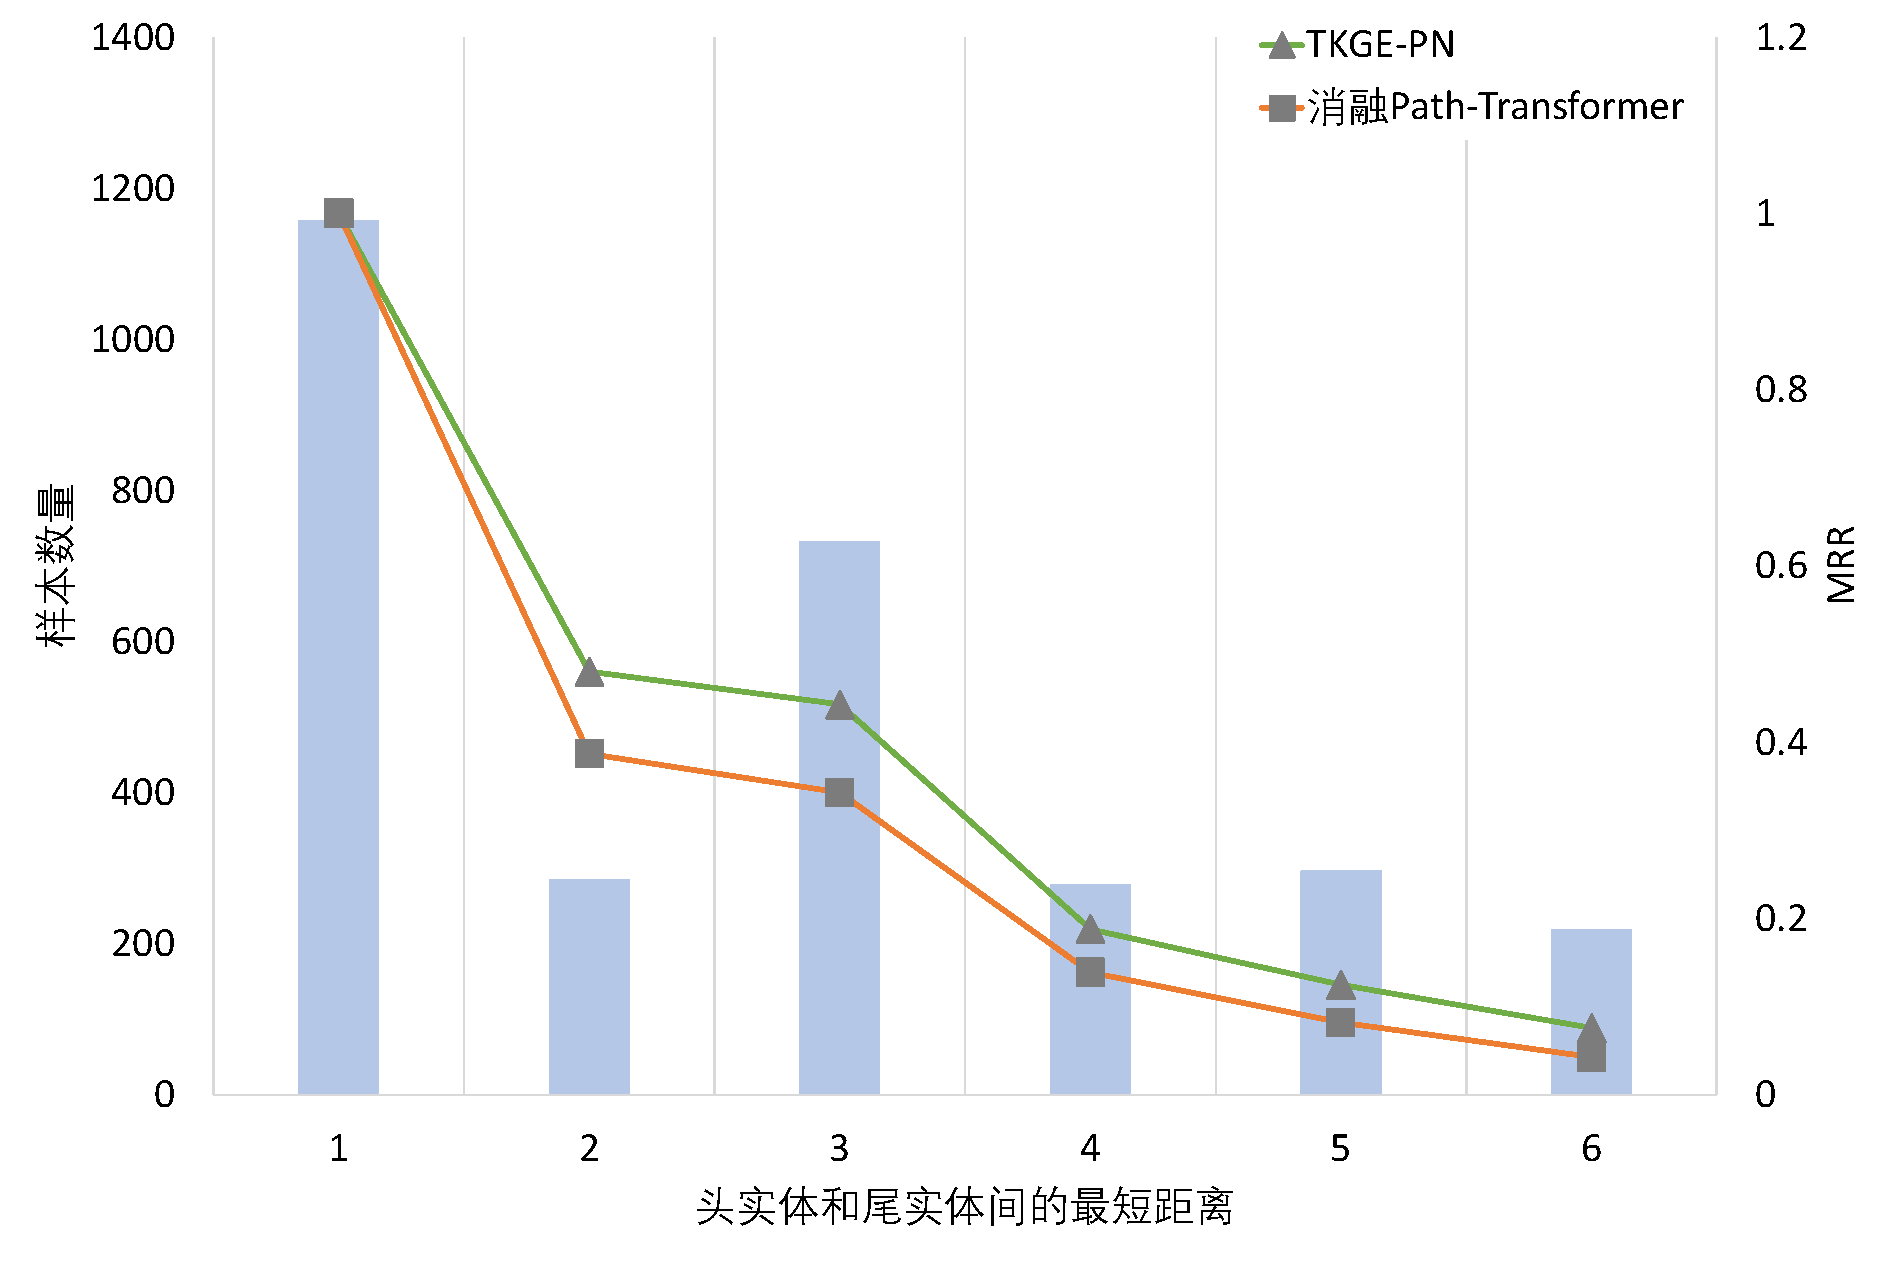
\includegraphics[width=0.75\textwidth]{pic/TKGE-PN_experiment.pdf}}
    \caption{WN18RR分组实验结果}
    \label{tkge_experiment}
  \end{figure}

从图\ref{tkge_experiment}中实验结果可以发现,随着头实体和尾实体之间最短距离的增加,模型的平均倒数排名MRR指标出现了明显的下降,进一步的说明推断图谱中实体之间的长距离关系是一件非常困难的任务。 此外,可以注意到的是,相比于消融了Path-Transformer图路径编码模块的模型,学习了图路径信息的原始TKGE-PN模型在长距离的样本上性能表现更好,特别是在头尾实体间最短距离为3-6的样本上,证明了知识图谱图路径信息能够帮助模型有效捕捉实体间的长距离依赖,推断实体间的长距离的关联,有效提高模型在部分场景下的知识图谱补全任务的性能表现。

\subsection{TKGE-PN模型超参数影响分析}

和NATLP类似,为了探究实体和关系嵌入维度对模型知识图谱补全任务性能的影响,本文在FB15k-237和WN18RR数据集的验证集上进行了实验,实体关系嵌入维度分别取$d \in \left[100,200,300,400,500\right] $,具体的实验结果如表\ref{dimension_2}所示。

\begin{table}[htbp]
    \begin{center}
        \caption{实体和关系嵌入维度对于TKGE-PN模型性能的影响}
        %\setlength{\tabcolsep}{12pt}
        \renewcommand{\arraystretch}{1.5}
        \begin{tabular}{*{5}{c}}
            \toprule
            嵌入维度& \multicolumn{2}{c}{WN18RR} & \multicolumn{2}{c}{FB15k-237}\\
            \cmidrule(lr){2-3}\cmidrule(lr){4-5}
            $d$&MRR&Hits@10&MRR&Hits@10\\
            \midrule
            100	&0.503&0.579&0.375&0.559\\
            200	&0.506&0.583&0.376&0.560\\
            300	&\textbf{0.509}&\textbf{0.587}&\textbf{0.379}&0.562\\
            400	&0.506&\textbf{0.587}&0.377&\textbf{0.563}\\
            500	&0.507&0.583&0.378&0.554\\
            \bottomrule
        \end{tabular}
        \label{dimension_2}
    \end{center}
\end{table}


从实验结果中可以观察到,总体而言,模型性能变化并不明显,证明了TKGE-PN模型的鲁棒性。另一方面,随着实体和关系嵌入维度的上升,模型性能呈现出先上升后下降的趋势。这是由于当嵌入维度较小时,TKGE-PN模型的表达能力会受到一定的限制,而在嵌入维度增大超过适宜范围后,参数量过大会导致计算复杂度提高,性能下降。

\section{本章小结}

本章首先对TKGE-PN模型的整体架构和实现细节进行了详细介绍。本文首先对基于图神经网络的方法以及前文提出的NATLP模型依然存在的问题进行了介绍;随后给出了模型中涉及到的数学符号的详细定义;之后介绍了模型的整体架构组成;最后,对TKGE-PN中的关键设计细节进行了具体的说明,包括(1)基于有偏随机游走的图路径采样算法,将图路径的路径深度以及实体的节点度数纳入了考虑,用于采样高质量的图路径(2)Path-Transformer路径编码模块,通过掩蔽实体关系预测任务加强模型学习图路径中语义信息的能力,实现了长短距离依赖信息的平衡(3)Neighbor-Transformer局部邻域编码模块,结合待预测的事实三元组,综合图路径结构信息和局部邻域结构信息完成链路预测任务。
而在实验部分,本文首先介绍了用来对比的基线模型及其特点,并说明了TKGE-PN模型在两个数据集上的超参数设置。之后论文对TKGE-PN模型的整体实验结果进行了说明,证明了TKGE-PN模型性能表现优于绝大部分现有的模型。论文随后通过实验进一步探究了路径长度以及路径采样策略对于TKGE-PN性能的影响;最后论文通过实验对TKGE-PN模型中的关键设计进行了具体的探究和分析,包括图路径编码模块、局部邻域编码模块以及掩蔽实体关系预测任务,并设计了实验证明了图路径在长距离依赖信息学习中的重要作用。
